%arara : pdflatex
\documentclass[•]{article}

\usepackage{../../TP0/style}

\begin{document}
\def\reportnumber{1}
\def\reporttitle{Mesure du temps d'exécution d'un programme.}
%----------------------------------------------------------------------------------------
%	TITLE PAGE
%----------------------------------------------------------------------------------------


\begin{titlepage} % Suppresses displaying the page number on the title page and the subsequent page counts as page 1
	\newcommand{\HRule}{\rule{\linewidth}{0.5mm}} % Defines a new command for horizontal lines, change thickness here
	
	\center % Centre everything on the page
	
	%------------------------------------------------
	%	Headings
	%------------------------------------------------
	
	\baselineskip=2\baselineskip 
	\textsc{\LARGE Université des Sciences et de la Technologie Houari Boumediene}%\\[1cm] % Main heading such as the name of your university/college

	%------------------------------------------------
	%	Logo
	%------------------------------------------------
	
	%\vfill\vfill
	\vfill
	
\includegraphics[width=0.3\textwidth]{../style/USTHB_Logo.png}\\[1cm] % Include a department/university logo - this will require the graphicx package
	 
	%----------------------------------------------------------------------------------------
	
	\textsc{\Large Compilation}\\[0.5cm] % Major heading such as course name
	%\textsc{\large Minor Heading}\\[0.5cm] % Minor heading such as course title
	
	%------------------------------------------------
	%	Title
	%------------------------------------------------
	
	\HRule\\[0.4cm]
	\baselineskip=1.2\baselineskip 
	{\huge\bfseries Rapport de Projet \\
	 \reporttitle}\\[0.4cm] % Title of your document
	
	\HRule\\[1.5cm]
	
	%------------------------------------------------
	%	Author(s)
	%------------------------------------------------
	
	\begin{minipage}{0.4\textwidth}
		\begin{flushleft}
			\large
			\textit{Binôme: groupe 4}\\
			HOUACINE  \textsc{Naila Aziza} % Your name
			\\
			MOHAMMEDI \textsc{Haroune } % Your name
			
		\end{flushleft}
	\end{minipage}
	~
	\begin{minipage}{0.4\textwidth}
		\begin{flushright}
			\large
			\textit{Professeur}\\
			Mme. MEKAHLIA \textsc{Fatma Zohra} % Supervisor's name
		\end{flushright}
	\end{minipage}
	
	%------------------------------------------------
	%	Date
	%------------------------------------------------
	
	\vfill\vfill\vfill % Position the date 3/4 down the remaining page
	
	{\large\today} % Date, change the \today to a set date if you want to be precise
	
	
	\vfill % Push the date up 1/4 of the remaining page
	
\end{titlepage}


\section{Partie I: Développement de l'algorithme et du programme pour le problème du calcul de la somme des n premiers nombres entiers naturels.}

\subsection{Développement de l'algorithme itératif qui permet de calculer la somme S des n premiers nombres entiers naturels.}
\textrm{L'écriture de ces algorithme sera accompagné de commentaire représentant le nombre de mot mémoire que prend chaque instruction puis celui de tous l'algorithme.}

\subsubsection{En utilisant la forme "pour ... faire":}
L'algorithme développé ci dessous, nommé Algorithme\_Somme\_Iteratif\_pour, utilise la forme de répétition : 

Pour ... faire ... fait.
\begin{sql}

 Algorithme_Somme_Iteratif_pour
 
 VAR
 i,N,S : entier;				//3 mots mémoire
 
 Debut
	ecrire("Donner N = ");		//1 mot mémoire
	lire(N);					//1 mot mémoire
	
	S = 0;						//1 mot mémoire
	
	pour(i=1 ; i <= N ; i++)	//4 mots mémoire
	  faire
		S = S + i;				//2 mots mémoire
	  fait;
	  
	ecrire("La somme = ",S);	//1 mot mémoire
	
 Fin.
\end{sql}
\textrm{Totale de mots mémoire = 13 MM}

\subsubsection{En utilisant la forme "tant que ... faire":}
\textrm{L algorithme développé ci dessous, nommé Algorithme\_Somme\_Iteratif\_tant\_que, utilise la forme de répétition : tant que ... faire ... fait.}
\begin{sql}

 Algorithme_Somme_Iteratif_tant_que
 
 VAR
 i,N,S : entier;				//3 mots mémoire
 
 Debut
	ecrire("Donner N = ");		//1 mot mémoire
	lire(N);					//1 mot mémoire
	
	S = 0;						//1 mot mémoire
	i = 1;						//1 mot mémoire
	
	tant que(i <= N)			//1 mot mémoire
	  faire
		S = S + i;				//2 mots mémoire
		i = i + 1;				//2 mots mémoire
	  fait;
	  
	ecrire("La somme = ",S);	//1 mot mémoire
	
 Fin.
\end{sql}
\textrm{Totale de mots mémoire = 13 MM}

\subsubsection{En utilisant la forme "répéter ... jusqu'à":}
\textrm{L algorithme développé ci dessous, nommé Algorithme\_Somme\_Iteratif\_répéter\_jusqu\_a, utilise la forme de répétition : répéter ... jusqu'à ...}
\begin{sql}

 Algorithme_Somme_Iteratif_répéter_jusqu_a
 
 VAR
 i,N,S : entier;				//3 mots mémoire
 
 Debut
	ecrire("Donner N = ");		//1 mot mémoire
	lire(N);					//1 mot mémoire
	
	S = 0;						//1 mot mémoire
	i = 1;						//1 mot mémoire
	
	répéter
		S = S + i;				//2 mots mémoire
		i = i + 1;				//2 mots mémoire
	  jusqu a(i > N);			//1 mot mémoire
	  
	ecrire("La somme = ",S);	//1 mot mémoire
	
 Fin.
\end{sql}
\textrm{Totale de mots mémoire = 13 MM}

\subsection{Développement des programmes itératifs en langage C.}
\subsubsection{En utilisant la forme "FOR":}
\begin{sql}
 #include<stdio.h>
 #include<stdlib.h> 
 
 int main()
 {
	long int i,N,S;
	
	printf("Donner N = ");
	scanf("%Ld",&N);
	
	S=0;
	
	for(i=1 ; i <= N ; i++)
	{
		S = S + i;
	}
	
	printf("La somme S = %Ld",S);
	return 0;
 }
\end{sql}

\subsubsection{En utilisant la forme "WHILE":}
\begin{sql}
 #include<stdio.h>
 #include<stdlib.h>
 
 int main()
 {
	long int i,N,S;
	
	printf("Donner N = ");
	scanf("%Ld",&N);
	
	S=0; i=1;
	
	while(i <= N)
	{
		S = S + i;
		i = i + 1;
	}
	
	printf("La somme S = %Ld",S);
	return 0;
 }
\end{sql}

\subsubsection{En utilisant la forme "DO ... WHILE":}
\begin{sql}
 #include<stdio.h>
 #include<stdlib.h>
 
 int main()
 {
	long int i,N,S;
	
	printf("Donner N = ");
	scanf("%Ld",&N);
	
	S=0; i=1;
	
	Do
	{
		S = S + i;
		i = i + 1;
	}while(i > N)
	
	printf("La somme S = %Ld",S);
	return 0;
 }
\end{sql}
\textrm{ }
\\

\subsection{Développement de l'algorithme récursif pour le problème.}

\begin{sql}
Procedure_Somme_Récursif(N , S : entier)
 
 VAR
 
 Debut									
 
	Si( N <= 0)										//1 mot mémoire
		Alors ecrire("La Somme S = ",S);			//1 mot mémoire
		Sinon   S = S + N;							//2 mots mémoire
				Algorithme_Somme_Récursif(N - 1,S);	//2 mots mémoire
	FinSi;
	
 Fin.
 
 
 Algorithme_Somme_Récursif()
 
 VAR
 
 Debut
	N: entier;										//1 mot mémoire

    ecrire("Donner N = ");							//1 mot mémoire
	lire(N);										//1 mot mémoire

	Procedure_Somme_Récursif(N , 0);				//1 mot mémoire
 Fin.
\end{sql}
\textrm{Totale de mots mémoire = 13 MM}

\subsection{Développement du programme récursif en langage C.}
\begin{sql}
 #include<stdio.h>
 #include<stdlib.h>

 void SommeRecursive(long int N,long int S)
 {
	if(N <= 0)
	{
		printf("La somme S = %Ld \n",S);
	}else
	{
		S = S + N;
		SommeRecursive(N - 1,S);
	}
 }


int main()
{
    long int N;

    printf("Donner N = ");
	scanf("%Ld",&N);

	SommeRecursive(N,0);

	return 0;
}

\end{sql}



\textrm{  }
\\

\section{Partie II: Mesure du temps d'exécution.}
\textrm{
Pour la mesure du temps en langage C nous aurons besoin des fonctions de la gestion du temps que l'on retrouve dans la bibliothèque time.h.}

\textrm{Donc nous devant d'abord inclure la directive \#include $<$time.h$>$
Puis définir deux(2) variables notées début et fin de type clock\_t.}

\textrm{A l'aide de la fonction "clock()" :
Récupéré le Temps avant l'exécution du programme dans début et
récupéré le Temps après la fin de l'exécution du programme dans fin.}
\textrm{Calculer la différence entre début et fin dans un variable nommé : Delta de type double.} 
\textrm{Afin que le temps d'exécution Delta soit donné en secondes, nous divisons ce dernier par le paramètre CLOCKS\_PER\_SEC.}



\subsection{Mesure des temps d'exécution et Représentation par un graphe}
Au lieu de mesurer séparément le temps d'exécution pour chaque valeur de n donnée, on automatise le processus des mesures en utilisant un tableau tab contenant toutes les valeurs à tester et affichant en boucle le résultat pour chaque valeur.
\subsubsection{L'algorithme itératif avec boucle FOR}
le programme

\begin{sql}
 #include<stdio.h>
 #include<stdlib.h>
 #include<math.h>
 #include<time.h>
 
 int main()
 {
 	double i,j,N,S;
	clock_t start_t, end_t;
    double total_t;
	 
	double tab[14]={pow(10,6),2*pow(10,6),pow(10,7),2*pow(10,7), pow(10,8), 2*pow(10,8),	pow(10,9), 2*pow(10,9), pow(10,10),2*pow(10,10), pow(10,11), 2*pow(10,11), pow(10,12), 2*pow(10,12)};
	
	printf("L'algorithme itératif avec boucle for \n\n");
	for(j=0 ; j < 14 ; j++) {
	
        start_t = clock();			/*debut*/
        
        S=0; i=1;
        
		for(i=1 ; i <= tab[(long int)j]; i++)
			 S = S + i;
		
        end_t = clock();			/*Fin*/
        
        printf("La somme S = %lf \n",S);
        total_t = (double) (end_t - start_t) / CLOCKS_PER_SEC;
        printf("pour %lf Iteration le programme prends %lf\n\n", tab[(long int)j], total_t);
    }
	return 0;
 }
\end{sql}

le tableau
\\
\\
\color{blue}
\begin{tabular}{ |p{2cm}||p{1.6cm}|p{1.6cm}|p{1.6cm}|p{1.6cm}|p{1.6cm}|p{1.6cm}|p{1.6cm}| }
 \hline
 Valeur N : & $10^6$& $2*10^6$& $10^7$& $2*10^7$& $10^8$& $2*10^8$& $10^9$ \\
 \hline
 Temps d'exe : & 0.011177 & 0.006160 & 0.031110 & 0.061784 & 0.308448 & 0.615293 &  3.076619 \\
 \hline
\end{tabular}
\\
\\
\\
\begin{tabular}{ |p{2cm}||p{1.6cm}|p{1.6cm}|p{1.6cm}|p{1.6cm}|p{1.6cm}|p{1.6cm}|p{1.6cm}| }
 \hline
 Valeur N : & $2*10^9$& $10^{10}$& $2*10^{10}$& $10^{11}$& $2*10^{11}$& $10^{12}$& $2*10^{12}$ \\
 \hline
 Temps d'exe : &  6.179196 & 30.920366 & 69.197337 & 314.129090 &718.460152 &3201.630410 & 6459.747801   \\
 \hline
\end{tabular}
\color{black}


\textrm{  }
\\

le graphe 
\textrm{  }
\\
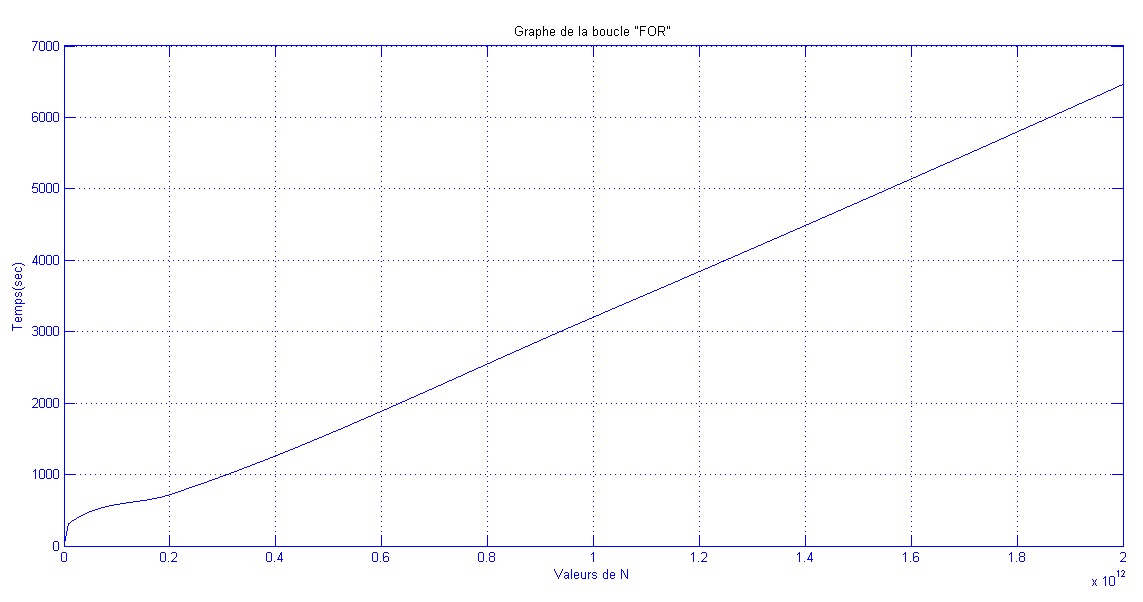
\includegraphics[width=1\textwidth]{graphe/for.png}


\subsubsection{L'algorithme itératif avec boucle while}
le programme
\begin{sql}
#include<stdio.h>
#include<stdlib.h>
#include <time.h>
#include <math.h>

 int main()
 {
 	double i,j,N,S;
	clock_t start_t, end_t;
    double total_t;
	 
	double tab[14]={pow(10,6),2*pow(10,6), pow(10,7),2*pow(10,7), pow(10,8), 2*pow(10,8),	pow(10,9), 2*pow(10,9), pow(10,10),2*pow(10,10), pow(10,11), 2*pow(10,11), pow(10,12), 2*pow(10,12)};
	
	printf("L'algorithme itératif avec boucle while \n\n");
	
	for(j=0 ; j < 14 ; j++) {
	
        start_t = clock();		/*debut*/
    
        
        S=0; i=1;
        
        while(i <= tab[(long int)j])
		{
			S = S + i;
			i = i + 1;
		}
		
        end_t = clock();		/*Fin*/
        
        printf("La somme S = %lf \n",S);
        total_t = (double) (end_t - start_t) / CLOCKS_PER_SEC;
        printf("pour %lf Iteration le programme prends %lf\n\n", tab[(long int)j], total_t);
    }
	return 0;
 }
\end{sql}

\textrm{  }

le tableau
\\
\\
\color{blue}
\begin{tabular}{ |p{2cm}||p{1.6cm}|p{1.6cm}|p{1.6cm}|p{1.6cm}|p{1.6cm}|p{1.6cm}|p{1.6cm}| }
 \hline

 Valeur N : & $10^6$& $2*10^6$& $10^7$& $2*10^7$& $10^8$& $2*10^8$& $10^9$ \\
 \hline
 Temps d'exe :  & 0.003227 & 0.006472 & 0.032436 & 0.064657 & 0.322734 & 0.646398 &  3.228527 \\
  
 \hline
\end{tabular}
\\
\\
\\
\begin{tabular}{ |p{2cm}||p{1.6cm}|p{1.6cm}|p{1.6cm}|p{1.6cm}|p{1.6cm}|p{1.6cm}|p{1.6cm}| }
 \hline
 Valeur N : & $2*10^9$& $10^{10}$& $2*10^{10}$& $10^{11}$& $2*10^{11}$& $10^{12}$& $2*10^{12}$ \\
 \hline
 Temps d'exe : &  6.456017 & 32.271228 & 67.204256 & 353.661353 & 709.004102 & 
 3640.236612 & 7196.518894   \\
 \hline
\end{tabular}
\color{black}

\textrm{  }
\\
\\

le graphe 

\textrm{  }
\\
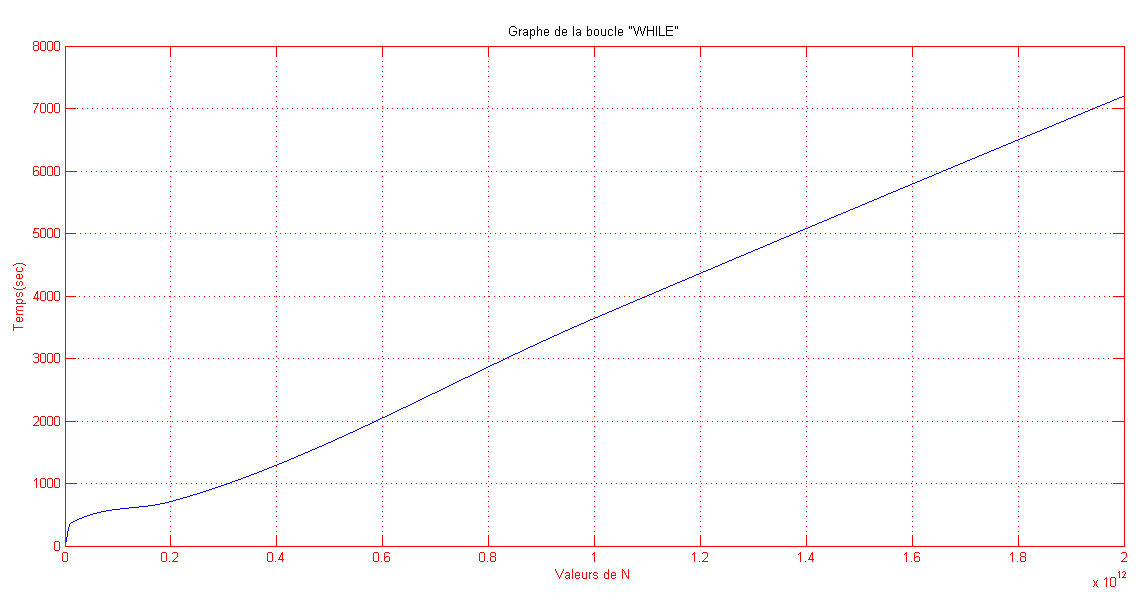
\includegraphics[width=1\textwidth]{graphe/while.png}
\\
\\
\\
\\
\\
\subsubsection{L'algorithme itératif avec boucle Do .. while}
le programme
\begin{sql}
#include <stdio.h>
#include <stdlib.h>
#include <time.h>
#include <math.h>

 int main()
 {
	double i,j,N,S;
	clock_t start_t, end_t;
    double total_t;
	 
	double tab[14]={pow(10,6),2*pow(10,6),pow(10,7),2*pow(10,7), pow(10,8), 2*pow(10,8), pow(10,9), 2*pow(10,9), pow(10,10),2*pow(10,10), pow(10,11), 2*pow(10,11), pow(10,12), 2*pow(10,12)};

	printf("L'algorithme itératif avec boucle do .. while \n\n");

	for(j=0 ; j < 14 ; j++) {

        start_t = clock();			/*debut*/
        
        S=0; i=1;

        do
        {
            S = S + i;
            i = i + 1;
        } while(i <= tab[(long int)j]);

        end_t = clock();			/*Fin*/

        printf("La somme S = %lf \n",S);
        total_t = (double) (end_t - start_t) / CLOCKS_PER_SEC;
        printf("pour %lf Iteration le programme prends %lf\n\n", tab[(long int)j], total_t);

    }
	return 0;
}
\end{sql}

\textrm{  }

le tableau
\\
\\
\color{blue}
\begin{tabular}{ |p{2cm}||p{1.6cm}|p{1.6cm}|p{1.6cm}|p{1.6cm}|p{1.6cm}|p{1.6cm}|p{1.6cm}| }
 \hline
 Valeur N : & $10^6$& $2*10^6$& $10^7$& $2*10^7$& $10^8$& $2*10^8$& $10^9$ \\
 \hline
 Temps d'exe : & 0.003294 & 0.006591 & 0.033344 & 0.066648 & 0.341006 & 0.692939 &  3.504640 \\
 \hline
\end{tabular}
\\
\\
\\
\begin{tabular}{ |p{2cm}||p{1.6cm}|p{1.6cm}|p{1.6cm}|p{1.6cm}|p{1.6cm}|p{1.6cm}|p{1.6cm}| }
\hline
Valeur N : & $2*10^9$& $10^{10}$& $2*10^{10}$& $10^{11}$& $2*10^{11}$& $10^{12}$& $2*10^{12}$ \\
 \hline
Temps d'exe : &  7.179120 & 35.645556 & 61.837564 & 317.164022 & 635.293616 & 3052.125339 & 6121.511236  \\
\hline
\end{tabular}

\color{black}

\textrm{  }
\\

le graphe 

\textrm{  }
\\
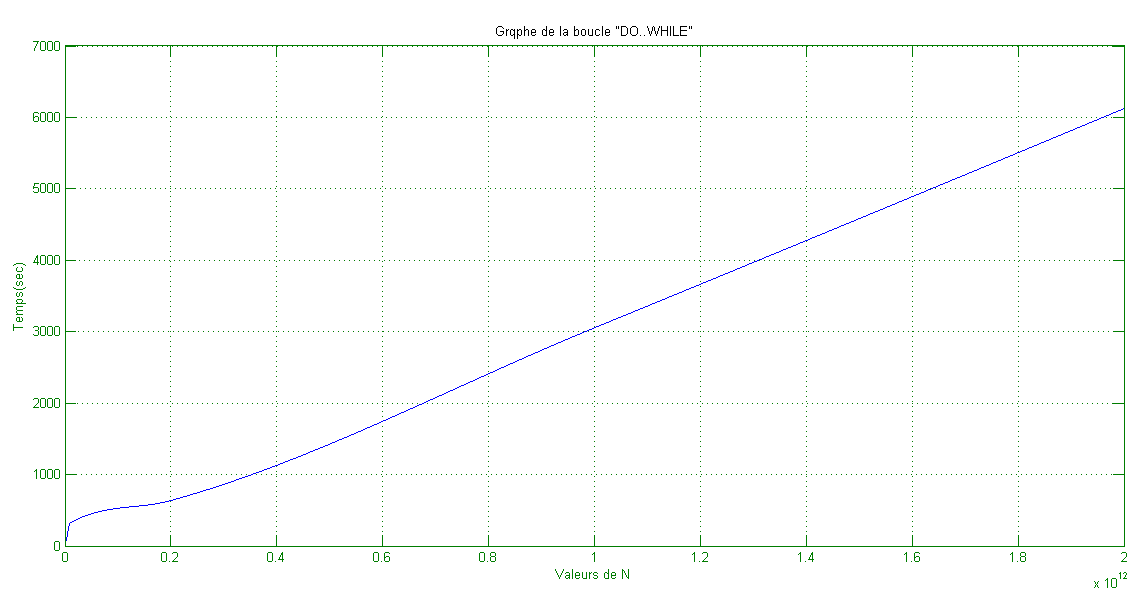
\includegraphics[width=1\textwidth]{graphe/do_while.png}

\subsubsection{L'algorithme récursif}

le programme

\begin{sql}
#include <stdio.h>
#include <stdlib.h>
#include <time.h>
#include <math.h>

void SommeRecursive(long int N, long int S)
{
	if(N > 0)
	{
		S = S + N;
		SommeRecursive(N - 1, S);
	}
	else{
        return;
	}

}


int main()
{

	long int i,j,N,S;
	clock_t start_t, end_t;
    double total_t;

	long int tab[14]={pow(10,6),2*pow(10,6),pow(10,7),2*pow(10,7),pow(10,8),2*pow(10,8),
	pow(10,9),2*pow(10,9),pow(10,10),2*pow(10,10),pow(10,11),2*pow(10,11),pow(10,12),2*pow(10,12)};

	printf("L'algorithme recursif\n");

	for(j=0 ; j < 14 ; j++) {

        start_t = clock();

        S=0; i=1;

        SommeRecursive(tab[(long int) j],S);

        end_t = clock();

        printf("La somme S = %lf \n",S);
        total_t = (double) (end_t - start_t) / CLOCKS_PER_SEC;
        printf("Pour N = %lf le programme prend %lf\n\n", tab[(long int) j], total_t);
    }


    return 0;
}

\end{sql}

\color{red}
Remarque: 
\color{black}
Les valeurs du tableau et le graphe correspondants à ce programme ne sont pas inclus dans ce rapport car les valeurs de N étant trop grandes conduisent à la saturation de la pile responsable de la gestion de la récursivité.

\textrm{ }
\\
\subsection{Déduction du temps d'exécution moyen}

1- On remarque que les valeurs et graphes obtenues avec les 3 algorithmes itératifs sont presque identiques;
donc il suffit d'étudier un seul, nous choisirons le programme utilisant la boucle WHILE.

2- On remarque que les temps d'exécution sont approximativement doublés lorsque N est doublé et qu'ils sont pratiquement multipliés par 10 lorsque N est multiplié par 10.
\\

\color{blue}
Exemples:
\color{black} 
\\
N = $10^{9} \rightarrow $  T = 3.228527
\\
N = $2*10^{9} \rightarrow $  T =  6.456017
\\

Aussi
\\
N = $10^{9} \rightarrow $  T = 3.228527
\\
N = $10^{10} = 10*10^{9} \rightarrow $  T =  32.271228
\\

3- On peut constater la linéarité du graphe. 
\\
\\
On en déduit que le temps d'exécution est proportionnel à N, ce que l'on peut représenter par la formule suivante
: 
\begin{center}

	$T(x*N) = x*T(N)$ pour tous $ x*N \in [10^6,2*10^{12} ] $	
	

(x étant la tangente d'un point sur le graphe).
\end{center}

Nous ne pouvant pas généraliser car les testes que nous avons fait n'englobent pas toutes les valeurs possibles, 
	la solution est le calcule de la complexité temporelle du programme.




\end{document}
